\chapter{File system}
\label{CH:FS}
%         is it process or kernel thread?
% 
%         the logging text (and some of the buffer text) assumes the reader
%         knows a fair amount about how inodes and directories work,
%         but they are introduced later.
% 
% 	have to decide on processor vs CPU, i/o vs I/O.
% 	
% 	be sure to say buffer, not block 
% 
% 	Mount

The purpose of a file system is to organize and store data. File systems
typically support sharing of data among users and applications, as well as
\indextext{persistence}
so that data is still available after a reboot.

The xv6 file system provides Unix-like files, directories, and pathnames
(see Chapter~\ref{CH:UNIX}), and stores its data on a virtio disk for
persistence (see Chapter~\ref{CH:TRAP}). The file system addresses
several challenges:
\begin{itemize}
  
\item The file system needs on-disk data structures to represent the tree
of named directories and files, to record the identities of the
blocks that hold each file's content, and to record which areas
of the disk are free.
\item The file system must support
\indextext{crash recovery}.
That is, if a crash (e.g., power failure) occurs, the file system must
still work correctly after a restart. The risk is that a crash might
interrupt a sequence of updates and leave inconsistent on-disk data
structures (e.g., a block that is both used in a file and marked free).
\item Different processes may operate on the file system at the same time,
so the file system code must coordinate to maintain invariants.
\item Accessing a disk is orders of magnitude slower than accessing
memory, so the file system must maintain an in-memory cache of
popular blocks.

\end{itemize}

The rest of this chapter explains how xv6 addresses these challenges.
%% 
%%  -------------------------------------------
%% 
\section{Overview}

The xv6 file system implementation is
organized in seven layers, shown in 
Figure~\ref{fig:fslayer}.
The disk layer reads and writes blocks on an virtio hard drive.
The buffer cache layer caches disk blocks and synchronizes access to them,
making sure that only one kernel process at a time can modify the
data stored in any particular block.  The logging layer allows higher
layers to wrap updates to several blocks in a
\indextext{transaction},
and ensures that the blocks are updated atomically in the
face of crashes (i.e., all of them are updated or none).
The inode layer provides individual files, each represented as an
\indextext{inode}
with a unique i-number
and some blocks holding the file's data.  The directory
layer implements each directory as a special kind of
inode whose content is a sequence of directory entries, each of which contains a
file's name and i-number.
The pathname layer provides
hierarchical path names like
\lstinline{/usr/rtm/xv6/fs.c},
and resolves them with recursive lookup.
The file descriptor layer abstracts many Unix resources (e.g., pipes, devices,
files, etc.) using the file system interface, simplifying the lives of
application programmers.

\begin{figure}[t]
\center
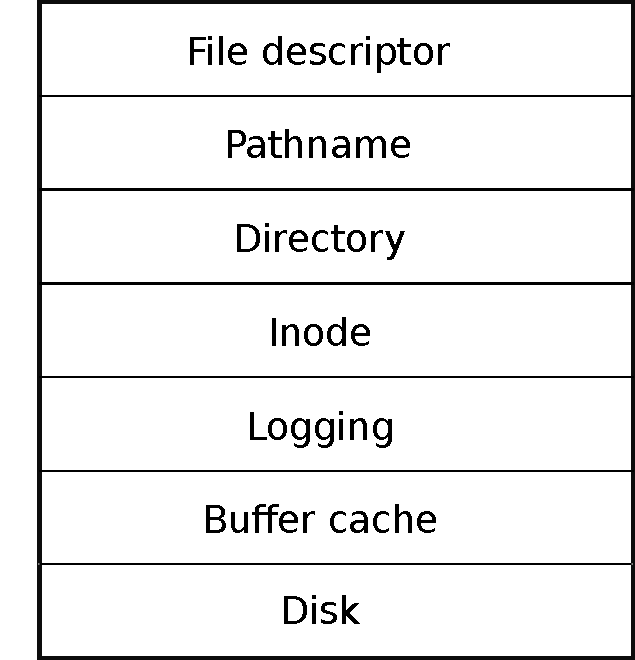
\includegraphics[scale=0.5]{fig/fslayer.pdf}
\caption{Layers of the xv6 file system.}
\label{fig:fslayer}
\end{figure}

The file system must have a plan for where it stores inodes and
content blocks on the disk.
To do so, xv6 divides the disk into several
sections, as shown in 
Figure~\ref{fig:fslayout}.
The file system does not use
block 0 (it holds the boot sector).  Block 1 is called the 
\indextext{superblock}; 
it contains metadata about the file system (the file system size in blocks, the
number of data blocks, the number of inodes, and the number of blocks in the
log).  Blocks starting at 2 hold the log.  After the log are the inodes, with multiple inodes per block.  After
those come bitmap blocks tracking which data blocks are in use.
The remaining blocks are data blocks; each is either marked
free in the bitmap block, or holds content for a file or directory.
The superblock is filled in by a separate program, called
\indexcode{mkfs},
which builds an initial file system.

The rest of this chapter discusses each layer, starting with the
buffer cache.
Look out for situations where well-chosen abstractions at lower layers
ease the design of higher ones.
%% 
%%  -------------------------------------------
%% 
\section{Buffer cache layer}

The buffer cache has two jobs: (1) synchronize access to disk blocks to ensure
that only one copy of a block is in memory and that only one kernel thread at a time
uses that copy; (2) cache popular blocks so that they don't need to be re-read from
the slow disk. The code is in
\lstinline{bio.c}.

The main interface exported by the buffer cache consists of
\indexcode{bread}
and
\indexcode{bwrite};
the former obtains a
\indextext{buf}
containing a copy of a block which can be read or modified in memory, and the
latter writes a modified buffer to the appropriate block on the disk.
A kernel thread must release a buffer by calling
\indexcode{brelse}
when it is done with it.
The buffer cache uses a per-buffer sleep-lock to ensure
that only one thread at a time uses each buffer
(and thus each disk block);
\lstinline{bread}
returns a locked buffer, and
\lstinline{brelse}
releases the lock.

Let's return to the buffer cache.
The buffer cache has a fixed number of buffers to hold disk blocks,
which means that if the file system asks for a block that is not
already in the cache, the buffer cache must recycle a buffer currently
holding some other block. The buffer cache recycles the
least recently used buffer for the new block. The assumption is that
the least recently used buffer is the one least likely to be used
again soon.

\begin{figure}[t]
\center
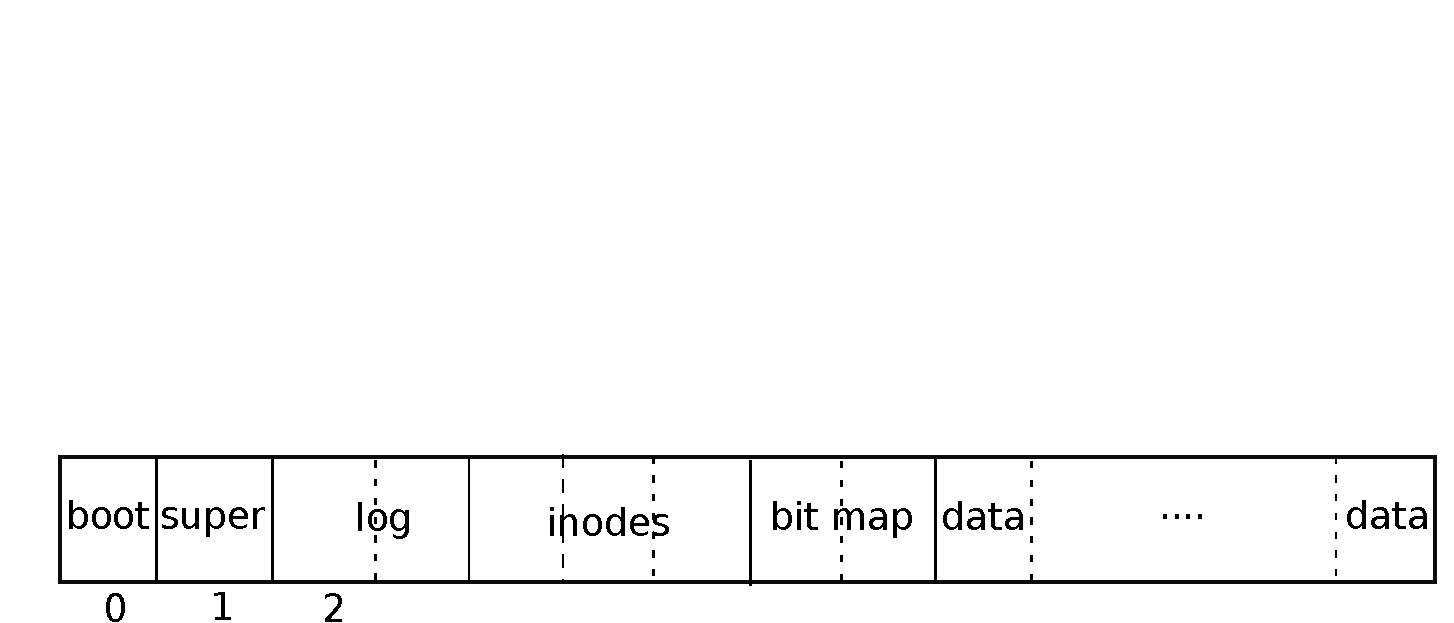
\includegraphics[scale=0.5]{fig/fslayout.pdf}
\caption{Structure of the xv6 file system. }
\label{fig:fslayout}
\end{figure}
%% 
%%  -------------------------------------------
%% 
\section{Code: Buffer cache}

The buffer cache is a doubly-linked list of buffers.
The function
\indexcode{binit},
called by
\indexcode{main}
\lineref{kernel/main.c:/binit/},
initializes the list with the
\indexcode{NBUF}
buffers in the static array
\lstinline{buf}
\linerefs{kernel/bio.c:/Create.linked.list/,/^..}/}.
All other access to the buffer cache refer to the linked list via
\indexcode{bcache.head},
not the
\lstinline{buf}
array.

A buffer has two state fields associated with it.
The field
\indexcode{valid}
indicates that the buffer contains a copy of the block.
The field \indexcode{disk}
indicates that the buffer content has been handed to
the disk, which may change the buffer (e.g., write
data from the disk into \lstinline{data}. 

\lstinline{Bread}
\lineref{kernel/bio.c:/^bread/}
calls
\indexcode{bget}
to get a buffer for the given sector
\lineref{kernel/bio.c:/b.=.bget/}.
If the buffer needs to be read from disk,
\lstinline{bread}
calls
\indexcode{virtio_disk_rw}
to do that before returning the buffer.

\lstinline{Bget}
\lineref{kernel/bio.c:/^bget/}
scans the buffer list for a buffer with the given device and sector numbers
\linerefs{kernel/bio.c:/Is.the.block.already/,/^..}/}.
If there is such a buffer,
\indexcode{bget}
acquires the sleep-lock for the buffer.
\lstinline{bget}
then returns the locked buffer.

If there is no cached buffer for the given sector,
\indexcode{bget}
must make one, possibly reusing a buffer that held
a different sector.
It scans the buffer list a second time, looking for a buffer
that is not in use (\lstinline{b->refcnt = 0}):
any such buffer can be used.
\lstinline{Bget}
edits the buffer metadata to record the new device and sector number
and acquires its sleep-lock.
Note that the assignment to
\lstinline{b->valid = 0}
ensures that
\lstinline{bread}
will read the block data from disk
rather than incorrectly using the buffer's previous contents.

It is important that there is at most one cached buffer per
disk sector, to ensure that readers see writes, and because the
file system uses locks on buffers for synchronization.
\lstinline{bget}
ensures this invariant by holding the
\lstinline{bache.lock}
continuously from the first loop's check of whether the
block is cached through the second loop's declaration that
the block is now cached (by setting
\lstinline{dev},
\lstinline{blockno},
and
\lstinline{refcnt}).
This causes the check for a block's presence and (if not
present) the designation of a buffer to hold the block to
be atomic.

It is safe for
\lstinline{bget}
to acquire the buffer's sleep-lock outside of the 
\lstinline{bcache.lock}
critical section,
since the non-zero
\lstinline{b->refcnt}
prevents the buffer from being re-used for a different disk block.
The sleep-lock protects reads
and writes of the block's buffered content, while the
\lstinline{bcache.lock}
protects information about which blocks are cached.

If all the buffers are busy, then too many processes are
simultaneously executing file system calls;
\lstinline{bget}
panics.
A more graceful response might be to sleep until a buffer became free,
though there would then be a possibility of deadlock.

Once
\indexcode{bread}
has read the disk (if needed) and returned the
buffer to its caller, the caller has
exclusive use of the buffer and can read or write the data bytes.
If the caller does modify the buffer, it must call
\indexcode{bwrite}
to write the changed data to disk before releasing the buffer.
\lstinline{Bwrite}
\lineref{kernel/bio.c:/^bwrite/}
calls
\indexcode{virtio_disk_rw}
to talk to the disk hardware.

When the caller is done with a buffer,
it must call
\indexcode{brelse}
to release it. 
(The name
\lstinline{brelse},
a shortening of
b-release,
is cryptic but worth learning:
it originated in Unix and is used in BSD, Linux, and Solaris too.)
\lstinline{Brelse}
\lineref{kernel/bio.c:/^brelse/}
releases the sleep-lock and
moves the buffer
to the front of the linked list
\linerefs{kernel/bio.c:/b->next->prev.=.b->prev/,/bcache.head.next.=.b/}.
Moving the buffer causes the
list to be ordered by how recently the buffers were used (meaning released):
the first buffer in the list is the most recently used,
and the last is the least recently used.
The two loops in
\lstinline{bget}
take advantage of this:
the scan for an existing buffer must process the entire list
in the worst case, but checking the most recently used buffers
first (starting at
\lstinline{bcache.head}
and following
\lstinline{next}
pointers) will reduce scan time when there is good locality of reference.
The scan to pick a buffer to reuse picks the least recently used
buffer by scanning backward
(following 
\lstinline{prev}
pointers).
%% 
%%  -------------------------------------------
%% 
\section{Logging layer}

One of the most interesting problems in file system design is crash
recovery. The problem arises because many file system operations
involve multiple writes to the disk, and a crash after a subset of the
writes may leave the on-disk file system in an inconsistent state. For
example, suppose a crash occurs during file truncation (setting
the length of a file to zero and freeing its content blocks).
Depending on the order of the disk writes, the crash 
may either leave an inode with a reference
to a content block that is marked free,
or it may leave an allocated but unreferenced content block.

The latter is relatively benign, but an inode that refers to a freed
block is likely to cause serious problems after a reboot.  After reboot, the
kernel might allocate that block to another file, and now we have two different
files pointing unintentionally to the same block.  If xv6 supported
multiple users, this situation could be a security problem, since the
old file's owner would be able to read and write blocks in the
new file, owned by a different user.

Xv6 solves the problem of crashes during file system operations with a
simple form of logging. An xv6 system call does not directly write
the on-disk file system data structures. Instead, it places a
description of all the disk writes it wishes to make in a 
\indextext{log} 
on the disk. Once the system call has logged all of its writes, it writes a
special 
\indextext{commit}
record to the disk indicating that the log contains
a complete operation. At that point the system call copies the writes
to the on-disk file system data structures. After those writes have
completed, the system call erases the log on disk.

If the system should crash and reboot, the file system code recovers
from the crash as follows, before running any processes. If the log is
marked as containing a complete operation, then the recovery code
copies the writes to where they belong in the on-disk file system. If
the log is not marked as containing a complete operation, the recovery
code ignores the log.  The recovery code finishes by erasing
the log.

Why does xv6's log solve the problem of crashes during file system
operations? If the crash occurs before the operation commits, then the
log on disk will not be marked as complete, the recovery code will
ignore it, and the state of the disk will be as if the operation had
not even started. If the crash occurs after the operation commits,
then recovery will replay all of the operation's writes, perhaps
repeating them if the operation had started to write them to the
on-disk data structure. In either case, the log makes operations
atomic with respect to crashes: after recovery, either all of the
operation's writes appear on the disk, or none of them appear.
%% 
%% 
%% 
\section{Log design}

The log resides at a known fixed location, specified in the superblock.
It consists of a header block followed by a sequence
of updated block copies (``logged blocks'').
The header block contains an array of sector
numbers, one for each of the logged blocks, and 
the count of log blocks.
The count in the header block on disk is either
zero, indicating that there is no transaction in the log,
or non-zero, indicating that the log contains a complete committed
transaction with the indicated number of logged blocks.
Xv6 writes the header
block when a transaction commits, but not before, and sets the
count to zero after copying the logged blocks to the file system.
Thus a crash midway through a transaction will result in a
count of zero in the log's header block; a crash after a commit
will result in a non-zero count.

Each system call's code indicates the start and end of the sequence of
writes that must be atomic with respect to crashes.
To allow concurrent execution of file system operations
by different processes,
the logging system can accumulate the writes
of multiple system calls into one transaction.
Thus a single commit may involve the writes of multiple
complete system calls.
To avoid splitting a system call across transactions, the logging system
only commits when no file system system calls are underway.

The idea of committing several transactions together is known as 
\indextext{group commit}.
Group commit reduces the number of disk operations
because it amortizes the fixed cost of a commit over multiple
operations.
Group commit also hands the disk system more concurrent writes
at the same time, perhaps allowing the disk to write
them all during a single disk rotation.
Xv6's virtio driver doesn't support this kind of
\indextext{batching},
but xv6's file system design allows for it.

Xv6 dedicates a fixed amount of space on the disk to hold the log.
The total number of blocks written by the system calls in a
transaction must fit in that space.
This has two consequences.
No single system call
can be allowed to write more distinct blocks than there is space
in the log. This is not a problem for most system calls, but two
of them can potentially write many blocks: 
\indexcode{write}
and
\indexcode{unlink}.
A large file write may write many data blocks and many bitmap blocks
as well as an inode block; unlinking a large file might write many
bitmap blocks and an inode.
Xv6's write system call breaks up large writes into multiple smaller
writes that fit in the log,
and 
\lstinline{unlink}
doesn't cause problems because in practice the xv6 file system uses
only one bitmap block.
The other consequence of limited log space
is that the logging system cannot allow a system call to start
unless it is certain that the system call's writes will
fit in the space remaining in the log.
%% 
%% 
%% 
\section{Code: logging}

A typical use of the log in a system call looks like this:
\begin{lstlisting}[]
  begin_op();
  ...
  bp = bread(...);
  bp->data[...] = ...;
  log_write(bp);
  ...
  end_op();
\end{lstlisting}

\indexcode{begin_op}
\lineref{kernel/log.c:/^begin.op/}
waits until
the logging system is not currently committing, and until
there is enough unreserved log space to hold
the writes from this call.
\lstinline{log.outstanding}
counts the number of system calls that have reserved log
space; the total reserved space is 
\lstinline{log.outstanding}
times
\lstinline{MAXOPBLOCKS}.
Incrementing
\lstinline{log.outstanding}
both reserves space and prevents a commit
from occuring during this system call.
The code conservatively assumes that each system call might write up to
\lstinline{MAXOPBLOCKS}
distinct blocks.

\indexcode{log_write}
\lineref{kernel/log.c:/^log.write/}
acts as a proxy for 
\indexcode{bwrite}.
It records the block's sector number in memory,
reserving it a slot in the log on disk,
and pins the buffer in the block cache
to prevent the block cache from evicting it.
The block must stay in the cache until committed:
until then, the cached copy is the only record
of the modification; it cannot be written to
its place on disk until after commit;
and other reads in the same transaction must
see the modifications.
\lstinline{log_write}
notices when a block is written multiple times during a single
transaction, and allocates that block the same slot in the log.
This optimization is often called
\indextext{absorption}.
It is common that, for example, the disk block containing inodes
of several files is written several times within a transaction.  By absorbing
several disk writes into one, the file system can save log space and
can achieve better performance because only one copy of the disk block must be
written to disk.

\indexcode{end_op}
\lineref{kernel/log.c:/^end.op/}
first decrements the count of outstanding system calls.
If the count is now zero, it commits the current
transaction by calling
\lstinline{commit().}
There are four stages in this process.
\lstinline{write_log()}
\lineref{kernel/log.c:/^write.log/}
copies each block modified in the transaction from the buffer
cache to its slot in the log on disk.
\lstinline{write_head()}
\lineref{kernel/log.c:/^write.head/}
writes the header block to disk: this is the
commit point, and a crash after the write will
result in recovery replaying the transaction's writes from the log.
\indexcode{install_trans}
\lineref{kernel/log.c:/^install_trans/}
reads each block from the log and writes it to the proper
place in the file system.
Finally
\lstinline{end_op}
writes the log header with a count of zero;
this has to happen before the next transaction starts writing
logged blocks, so that a crash doesn't result in recovery
using one transaction's header with the subsequent transaction's
logged blocks.

\indexcode{recover_from_log}
\lineref{kernel/log.c:/^recover_from_log/}
is called from 
\indexcode{initlog}
\lineref{kernel/log.c:/^initlog/},
which is called from \indexcode{fsinit}\lineref{kernel/fs.c:/^fsinit/} during boot before the first user process runs
\lineref{kernel/proc.c:/fsinit/}.
It reads the log header, and mimics the actions of
\lstinline{end_op}
if the header indicates that the log contains a committed transaction.

An example use of the log occurs in 
\indexcode{filewrite}
\lineref{kernel/file.c:/^filewrite/}.
The transaction looks like this:
\begin{lstlisting}[]
      begin_op();
      ilock(f->ip);
      r = writei(f->ip, ...);
      iunlock(f->ip);
      end_op();
\end{lstlisting}
This code is wrapped in a loop that breaks up large writes into individual
transactions of just a few sectors at a time, to avoid overflowing
the log.  The call to
\indexcode{writei}
writes many blocks as part of this
transaction: the file's inode, one or more bitmap blocks, and some data
blocks.
%% 
%% 
%% 
\section{Code: Block allocator}

File and directory content is stored in disk blocks,
which must be allocated from a free pool.
xv6's block allocator
maintains a free bitmap on disk, with one bit per block. 
A zero bit indicates that the corresponding block is free;
a one bit indicates that it is in use.
The program
\lstinline{mkfs}
sets the bits corresponding to the boot sector, superblock, log blocks, inode
blocks, and bitmap blocks.

The block allocator provides two functions:
\indexcode{balloc}
allocates a new disk block, and
\indexcode{bfree}
frees a block.
\lstinline{Balloc}
The loop in
\lstinline{balloc}
at
\lineref{kernel/fs.c:/^..for.b.=.0/}
considers every block, starting at block 0 up to 
\lstinline{sb.size},
the number of blocks in the file system.
It looks for a block whose bitmap bit is zero,
indicating that it is free.
If
\lstinline{balloc}
finds such a block, it updates the bitmap 
and returns the block.
For efficiency, the loop is split into two 
pieces.
The outer loop reads each block of bitmap bits.
The inner loop checks all 
\lstinline{BPB}
bits in a single bitmap block.
The race that might occur if two processes try to allocate
a block at the same time is prevented by the fact that
the buffer cache only lets one process use any one bitmap block at a time.

\lstinline{Bfree}
\lineref{kernel/fs.c:/^bfree/}
finds the right bitmap block and clears the right bit.
Again the exclusive use implied by
\lstinline{bread}
and
\lstinline{brelse}
avoids the need for explicit locking.

As with much of the code described in the remainder of this chapter, 
\lstinline{balloc}
and
\lstinline{bfree}
must be called inside a transaction.
%% 
%%  -------------------------------------------
%% 
\section{Inode layer}

The term 
\indextext{inode} 
can have one of two related meanings.
It might refer to the on-disk data structure containing
a file's size and list of data block numbers.
Or ``inode'' might refer to an in-memory inode, which contains
a copy of the on-disk inode as well as extra information needed
within the kernel.

The on-disk inodes
are packed into a contiguous area
of disk called the inode blocks.
Every inode is the same size, so it is easy, given a
number n, to find the nth inode on the disk.
In fact, this number n, called the inode number or i-number,
is how inodes are identified in the implementation.

The on-disk inode is defined by a
\indexcode{struct dinode}
\lineref{kernel/fs.h:/^struct.dinode/}.
The 
\lstinline{type}
field distinguishes between files, directories, and special
files (devices).
A type of zero indicates that an on-disk inode is free.
The
\lstinline{nlink}
field counts the number of directory entries that
refer to this inode, in order to recognize when the
on-disk inode and its data blocks should be freed.
The
\lstinline{size}
field records the number of bytes of content in the file.
The
\lstinline{addrs}
array records the block numbers of the disk blocks holding
the file's content.

The kernel keeps the set of active inodes in memory;
\indexcode{struct inode}
\lineref{kernel/file.h:/^struct.inode/}
is the in-memory copy of a 
\lstinline{struct}
\lstinline{dinode}
on disk.
The kernel stores an inode in memory only if there are
C pointers referring to that inode. The
\lstinline{ref}
field counts the number of C pointers referring to the
in-memory inode, and the kernel discards the inode from
memory if the reference count drops to zero.
The
\indexcode{iget}
and
\indexcode{iput}
functions acquire and release pointers to an inode,
modifying the reference count.
Pointers to an inode can come from file descriptors,
current working directories, and transient kernel code
such as
\lstinline{exec}.

There are four lock or lock-like mechanisms in xv6's
inode code.
\lstinline{icache.lock}
protects the invariant that an inode is present in the cache
at most once, and the invariant that a cached inode's
\lstinline{ref}
field counts the number of in-memory pointers to the cached inode.
Each in-memory inode has a
\lstinline{lock}
field containing a
sleep-lock, which ensures exclusive access to the
inode's fields (such as file length) as well as to the
inode's file or directory content blocks.
An inode's
\lstinline{ref},
if it is greater than zero, causes the system to maintain
the inode in the cache, and not re-use the cache entry for
a different inode.
Finally, each inode contains a
\lstinline{nlink}
field (on disk and copied in memory if it is cached) that
counts the number of directory entries that refer to a file;
xv6 won't free an inode if its link count is greater than zero.

A
\lstinline{struct}
\lstinline{inode}
pointer returned by
\lstinline{iget()}
is guaranteed to be valid until the corresponding call to
\lstinline{iput()};
the inode won't be deleted, and the memory referred to
by the pointer won't be re-used for a different inode.
\lstinline{iget()}
provides non-exclusive access to an inode, so that
there can be many pointers to the same inode.
Many parts of the file system code depend on this behavior of
\lstinline{iget()},
both to hold long-term references to inodes (as open files
and current directories) and to prevent races while avoiding
deadlock in code that manipulates multiple inodes (such as
pathname lookup).

The
\lstinline{struct}
\lstinline{inode}
that 
\lstinline{iget}
returns may not have any useful content.
In order to ensure it holds a copy of the on-disk
inode, code must call
\indexcode{ilock}.
This locks the inode (so that no other process can
\lstinline{ilock}
it) and reads the inode from the disk,
if it has not already been read.
\lstinline{iunlock}
releases the lock on the inode.
Separating acquisition of inode pointers from locking
helps avoid deadlock in some situations, for example during
directory lookup.
Multiple processes can hold a C pointer to an inode
returned by 
\lstinline{iget},
but only one process can lock the inode at a time.

The inode cache only caches inodes to which kernel code
or data structures hold C pointers.
Its main job is really synchronizing access by multiple processes;
caching is secondary.
If an inode is used frequently, the buffer cache will probably
keep it in memory if it isn't kept by the inode cache.
The inode cache is \indextext{write-through}, which means that code that
modifies a cached inode must immediately write it to disk with
\lstinline{iupdate}.
%% 
%%  -------------------------------------------
%% 
\section{Code: Inodes}

To allocate a new inode (for example, when creating a file),
xv6 calls
\indexcode{ialloc}
\lineref{kernel/fs.c:/^ialloc/}.
\lstinline{Ialloc}
is similar to
\indexcode{balloc}:
it loops over the inode structures on the disk, one block at a time,
looking for one that is marked free.
When it finds one, it claims it by writing the new 
\lstinline{type}
to the disk and then returns an entry from the inode cache
with the tail call to 
\indexcode{iget}
\lineref{kernel/fs.c:/return.iget\(dev..inum\)/}.
The correct operation of
\lstinline{ialloc}
depends on the fact that only one process at a time
can be holding a reference to 
\lstinline{bp}:
\lstinline{ialloc}
can be sure that some other process does not
simultaneously see that the inode is available
and try to claim it.

\lstinline{Iget}
\lineref{kernel/fs.c:/^iget/}
looks through the inode cache for an active entry (\lstinline{ip->ref}
\lstinline{>}
\lstinline{0})
with the desired device and inode number.
If it finds one, it returns a new reference to that inode
\linerefs{kernel/fs.c:/^....if.ip->ref.>.0/,/^....}/}.
As
\indexcode{iget}
scans, it records the position of the first empty slot
\linerefs{kernel/fs.c:/^....if.empty.==.0/,/empty.=.ip/},
which it uses if it needs to allocate a cache entry.

Code must lock the inode using
\indexcode{ilock}
before reading or writing its metadata or content.
\lstinline{Ilock}
\lineref{kernel/fs.c:/^ilock/}
uses a sleep-lock for this purpose.
Once
\indexcode{ilock}
has exclusive access to the inode, it reads the inode
from disk (more likely, the buffer cache) if needed.
The function
\indexcode{iunlock}
\lineref{kernel/fs.c:/^iunlock/}
releases the sleep-lock,
which may cause any processes sleeping
to be woken up.

\lstinline{Iput}
\lineref{kernel/fs.c:/^iput/}
releases a C pointer to an inode
by decrementing the reference count
\lineref{kernel/fs.c:/^..ip->ref--/}.
If this is the last reference, the inode's
slot in the inode cache is now free and can be re-used
for a different inode.

If 
\indexcode{iput}
sees that there are no C pointer references to an inode
and that the inode has no links to it (occurs in no
directory), then the inode and its data blocks must
be freed.
\lstinline{Iput}
calls
\indexcode{itrunc}
to truncate the file to zero bytes, freeing the data blocks;
sets the inode type to 0 (unallocated);
and writes the inode to disk
\lineref{kernel/fs.c:/inode.has.no.links.and/}.

The locking protocol in 
\indexcode{iput}
in the case in which it frees the inode deserves a closer look.
One danger is that a concurrent thread might be waiting in
\lstinline{ilock}
to use this inode (e.g. to read a file or list a directory),
and won't be prepared to find the inode is not longer
allocated. This can't happen because there is no way for
a system call to get a pointer to a cached inode if it has
no links to it and 
\lstinline{ip->ref}
is one. That one reference is the reference owned by the
thread calling
\lstinline{iput}.
It's true that 
\lstinline{iput}
checks that the reference count is one outside of its
\lstinline{icache.lock}
critical section, but at that point the link
count is known to be zero, so no thread will try
to acquire a new reference.
The other main danger is that a concurrent call to
\lstinline{ialloc}
might choose the same inode that
\lstinline{iput}
is freeing.
This can only happen after the
\lstinline{iupdate}
writes the disk so that the inode has type zero.
This race is benign; the allocating thread will politely wait
to acquire the inode's sleep-lock before reading or writing
the inode, at which point
\lstinline{iput}
is done with it.

\lstinline{iput()}
can write to the disk.  This means that any system call that uses the file
system may write the disk, because the system call may be the last one having a
reference to the file. Even calls like
\lstinline{read()}
that appear to be read-only, may end up calling
\lstinline{iput().}
This, in turn, means that even read-only system calls
must be wrapped in transactions if they use the file system.

There is a challenging interaction between
\lstinline{iput()}
and crashes.
\lstinline{iput()}
doesn't truncate a file immediately when the link count for the file
drops to zero, because some process might still hold a reference to the inode in
memory: a process might still be reading and writing to the file, because it
successfully opened it. But, if a crash happens before the last process closes
the file descriptor for the file, then the file will be marked allocated on disk
but no directory entry points to it.

File systems handle this case in one of two ways. The simple solution is that on
recovery, after reboot, the file system scans the whole file system for files
that are marked allocated, but have no directory entry pointing to them.  If any
such file exists, then it can free those files.

The second solution doesn't require scanning the file system.  In this solution,
the file system records on disk (e.g., in the super block) the inode inumber of
a file whose link count drops to zero but whose reference count isn't zero.  If
the file system removes the file when its reference counts reaches 0, then it
updates the on-disk list by removing that inode from the list. On recovery, the
file system frees any file in the list.

Xv6 implements neither solution, which means that inodes may be marked allocated
on disk, even though they are not in use anymore.  This means that over time xv6
runs the risk that it may run out of disk space.
%% 
%% 
%% 
\section{Code: Inode content}

\begin{figure}[t]
\center
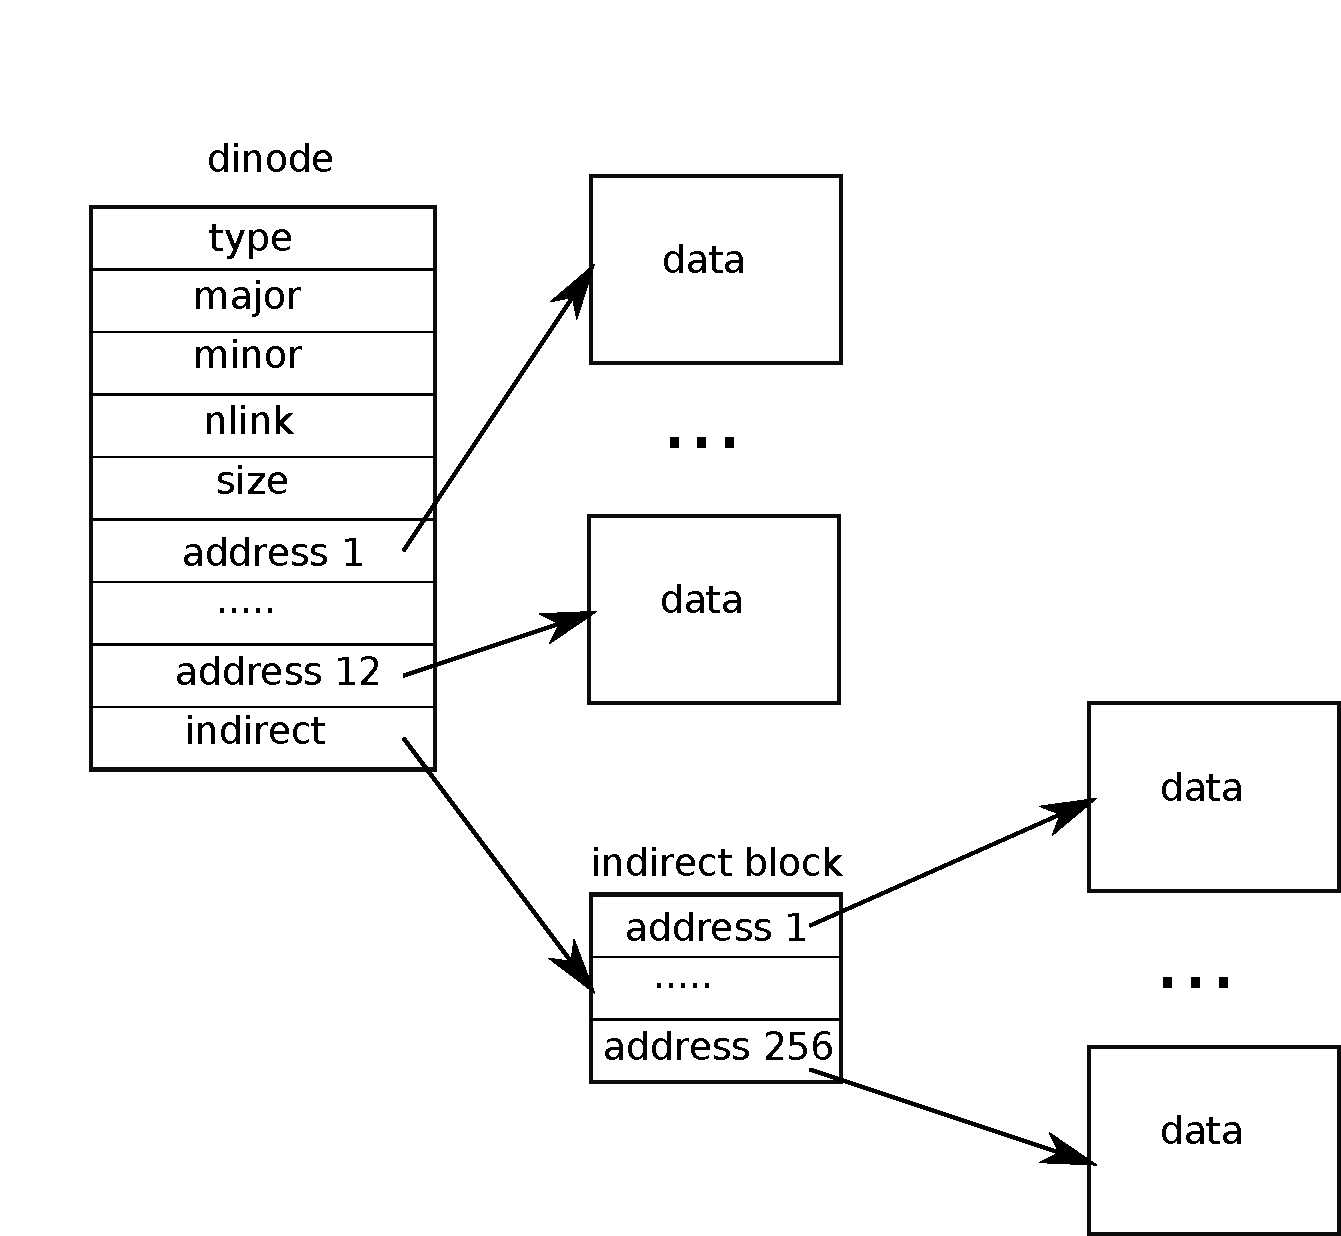
\includegraphics[scale=0.5]{fig/inode.pdf}
\caption{The representation of a file on disk.}
\label{fig:inode}
\end{figure}

The on-disk inode structure,
\indexcode{struct dinode},
contains a size and an array of block numbers (see 
Figure~\ref{fig:inode}).
The inode data is found in the blocks listed
in the
\lstinline{dinode} 's
\lstinline{addrs}
array.
The first
\indexcode{NDIRECT}
blocks of data are listed in the first
\lstinline{NDIRECT}
entries in the array; these blocks are called 
\indextext{direct blocks}.
The next 
\indexcode{NINDIRECT}
blocks of data are listed not in the inode
but in a data block called the
\indextext{indirect block}.
The last entry in the
\lstinline{addrs}
array gives the address of the indirect block.
Thus the first 12 kB (
\lstinline{NDIRECT} 
\lstinline{x}
\indexcode{BSIZE})
bytes of a file can be loaded from blocks listed in the inode,
while the next
\lstinline{256} kB (
\lstinline{NINDIRECT}
\lstinline{x}
\lstinline{BSIZE})
bytes can only be loaded after consulting the indirect block.
This is a good on-disk representation but a 
complex one for clients.
The function
\indexcode{bmap}
manages the representation so that higher-level routines such as
\indexcode{readi}
and
\indexcode{writei},
which we will see shortly.
\lstinline{Bmap}
returns the disk block number of the
\lstinline{bn} 'th
data block for the inode
\lstinline{ip}.
If
\lstinline{ip}
does not have such a block yet,
\lstinline{bmap}
allocates one.

The function
\indexcode{bmap}
\lineref{kernel/fs.c:/^bmap/}
begins by picking off the easy case: the first 
\indexcode{NDIRECT}
blocks are listed in the inode itself
\linerefs{kernel/fs.c:/^..if.bn.<.NDIRECT/,/^..}/}.
The next 
\indexcode{NINDIRECT}
blocks are listed in the indirect block at
\lstinline{ip->addrs[NDIRECT]}.
\lstinline{Bmap}
reads the indirect block
\lineref{kernel/fs.c:/bp.=.bread.ip->dev..addr/}
and then reads a block number from the right 
position within the block
\lineref{kernel/fs.c:/a.=..uint\*.bp->data/}.
If the block number exceeds
\lstinline{NDIRECT}+NINDIRECT,
\lstinline{bmap} 
panics; 
\lstinline{writei}
contains the check that prevents this from happening
\lineref{kernel/fs.c:/off...n...MAXFILE.BSIZE/}.

\lstinline{Bmap}
allocates blocks as needed.
An
\lstinline{ip->addrs[]}
or indirect
entry of zero indicates that no block is allocated.
As
\lstinline{bmap}
encounters zeros, it replaces them with the numbers of fresh blocks,
allocated on demand
\linerefs{kernel/fs.c:/^....if..addr.=.*==.0/,/./}
\linerefs{kernel/fs.c:/^....if..addr.*NDIRECT.*==.0/,/./}.

\indexcode{itrunc}
frees a file's blocks, resetting the inode's size to zero.
\lstinline{Itrunc}
\lineref{kernel/fs.c:/^itrunc/}
starts by freeing the direct blocks
\linerefs{kernel/fs.c:/^..for.i.=.0.*NDIRECT/,/^..}/},
then the ones listed in the indirect block
\linerefs{kernel/fs.c:/^....for.j.=.0.*NINDIRECT/,/^....}/},
and finally the indirect block itself
\linerefs{kernel/fs.c:/^....bfree.*NDIRECT/,/./}.

\lstinline{Bmap}
makes it easy for
\indexcode{readi}
and
\indexcode{writei} 
to get at an inode's data.
\lstinline{Readi}
\lineref{kernel/fs.c:/^readi/}
starts by
making sure that the offset and count are not 
beyond the end of the file.
Reads that start beyond the end of the file return an error
\linerefs{kernel/fs.c:/^..if.off.>.ip->size/,/./}
while reads that start at or cross the end of the file 
return fewer bytes than requested
\linerefs{kernel/fs.c:/^..if.off.\+.n.>.ip->size/,/./}.
The main loop processes each block of the file,
copying data from the buffer into 
\lstinline{dst}
\linerefs{kernel/fs.c:/^..for.tot=0/,/^..}/}.
%%  NOTE: It is very hard to write line references
%%  for writei because so many of the lines are identical
%%  to those in readi.  Luckily, identical lines probably
%%  don't need to be commented upon.
\indexcode{writei}
\lineref{kernel/fs.c:/^writei/}
is identical to
\indexcode{readi},
with three exceptions:
writes that start at or cross the end of the file
grow the file, up to the maximum file size
\linerefs{kernel/fs.c:/^..if.off.\+.n.>.MAXFILE/,/./};
the loop copies data into the buffers instead of out
\lineref{kernel/fs.c:/memmove.*bp->data/};
and if the write has extended the file,
\indexcode{writei}
must update its size
\linerefs{kernel/fs.c:/^..if.n.>.0.*off.>.ip->size/,/^..}/}.

Both
\indexcode{readi}
and
\indexcode{writei}
begin by checking for
\lstinline{ip->type}
\lstinline{==}
\indexcode{T_DEV}.
This case handles special devices whose data does not
live in the file system; we will return to this case in the file descriptor layer.

The function
\indexcode{stati}
\lineref{kernel/fs.c:/^stati\(/}
copies inode metadata into the 
\lstinline{stat}
structure, which is exposed to user programs
via the
\indexcode{stat}
system call.
%% 
%% 
%% 
\section{Code: directory layer}

A directory is implemented internally much like a file.
Its inode has type
\indexcode{T_DIR}
and its data is a sequence of directory entries.
Each entry is a
\indexcode{struct dirent}
\lineref{kernel/fs.h:/^struct.dirent/},
which contains a name and an inode number.
The name is at most
\indexcode{DIRSIZ}
(14) characters;
if shorter, it is terminated by a NUL (0) byte.
Directory entries with inode number zero are free.

The function
\indexcode{dirlookup}
\lineref{kernel/fs.c:/^dirlookup/}
searches a directory for an entry with the given name.
If it finds one, it returns a pointer to the corresponding inode, unlocked,
and sets 
\lstinline{*poff}
to the byte offset of the entry within the directory,
in case the caller wishes to edit it.
If
\lstinline{dirlookup}
finds an entry with the right name,
it updates
\lstinline{*poff}
and returns an unlocked inode
obtained via
\indexcode{iget}.
\lstinline{Dirlookup}
is the reason that 
\lstinline{iget}
returns unlocked inodes.
The caller has locked
\lstinline{dp},
so if the lookup was for
\indexcode{.},
an alias for the current directory,
attempting to lock the inode before
returning would try to re-lock
\lstinline{dp}
and deadlock.
(There are more complicated deadlock scenarios involving
multiple processes and
\indexcode{..},
an alias for the parent directory;
\lstinline{.}
is not the only problem.)
The caller can unlock
\lstinline{dp}
and then lock
\lstinline{ip},
ensuring that it only holds one lock at a time.

The function
\indexcode{dirlink}
\lineref{kernel/fs.c:/^dirlink/}
writes a new directory entry with the given name and inode number into the
directory
\lstinline{dp}.
If the name already exists,
\lstinline{dirlink}
returns an error
\linerefs{kernel/fs.c:/Check.that.name.is.not.present/,/^..}/}.
The main loop reads directory entries looking for an unallocated entry.
When it finds one, it stops the loop early
\linerefs{kernel/fs.c:/^....if.de.inum.==.0/,/./},
with 
\lstinline{off}
set to the offset of the available entry.
Otherwise, the loop ends with
\lstinline{off}
set to
\lstinline{dp->size}.
Either way, 
\lstinline{dirlink}
then adds a new entry to the directory
by writing at offset
\lstinline{off}
\linerefs{kernel/fs.c:/^..strncpy/,/panic/}.
%% 
%% 
%% 
\section{Code: Path names}

Path name lookup involves a succession of calls to
\indexcode{dirlookup},
one for each path component.
\lstinline{Namei}
\lineref{kernel/fs.c:/^namei/}
evaluates 
\lstinline{path}
and returns the corresponding 
\lstinline{inode}.
The function
\indexcode{nameiparent}
is a variant: it stops before the last element, returning the 
inode of the parent directory and copying the final element into
\lstinline{name}.
Both call the generalized function
\indexcode{namex}
to do the real work.

\lstinline{Namex}
\lineref{kernel/fs.c:/^namex/}
starts by deciding where the path evaluation begins.
If the path begins with a slash, evaluation begins at the root;
otherwise, the current directory
\linerefs{kernel/fs.c:/..if.\*path.==....\)/,/idup/}.
Then it uses
\indexcode{skipelem}
to consider each element of the path in turn
\lineref{kernel/fs.c:/while.*skipelem/}.
Each iteration of the loop must look up 
\lstinline{name}
in the current inode
\lstinline{ip}.
The iteration begins by locking
\lstinline{ip}
and checking that it is a directory.
If not, the lookup fails
\linerefs{kernel/fs.c:/^....ilock.ip/,/^....}/}.
(Locking
\lstinline{ip}
is necessary not because 
\lstinline{ip->type}
can change underfoot—it can't—but because
until 
\indexcode{ilock}
runs,
\lstinline{ip->type}
is not guaranteed to have been loaded from disk.)
If the call is 
\indexcode{nameiparent}
and this is the last path element, the loop stops early,
as per the definition of
\lstinline{nameiparent};
the final path element has already been copied
into
\lstinline{name},
so
\indexcode{namex}
need only
return the unlocked
\lstinline{ip}
\linerefs{kernel/fs.c:/^....if.nameiparent/,/^....}/}.
Finally, the loop looks for the path element using
\indexcode{dirlookup}
and prepares for the next iteration by setting
\lstinline{ip = next}
\linerefs{kernel/fs.c:/^....if..next.*dirlookup/,/^....ip.=.next/}.
When the loop runs out of path elements, it returns
\lstinline{ip}.

The procedure
\lstinline{namex}
may take a long time to complete: it could involve several disk operations to
read inodes and directory blocks for the directories traversed in the pathname
(if they are not in the buffer cache).  Xv6 is carefully designed so that if an
invocation of
\lstinline{namex}
by one kernel thread is blocked on a disk I/O, another kernel thread looking up
a different pathname can proceed concurrently.
\lstinline{namex}
locks each directory in the path separately so that lookups in different
directories can proceed in parallel.

This concurrency introduces some challenges. For example, while one kernel
thread is looking up a pathname another kernel thread may be changing the
directory tree by unlinking a directory.  A potential risk is that a lookup
may be searching a directory that has been deleted by another kernel thread and
its blocks have been re-used for another directory or file.

Xv6 avoids such races.  For example, when executing
\lstinline{dirlookup}
in
\lstinline{namex},
the lookup thread holds the lock on the directory and
\lstinline{dirlookup}
returns an inode that was obtained using
\lstinline{iget}.
\lstinline{iget}
increases the reference count of the inode.  Only after receiving the
inode from
\lstinline{dirlookup}
does
\lstinline{namex}
release the lock on the directory.  Now another thread may unlink the inode from
the directory but xv6 will not delete the inode yet, because the reference count
of the inode is still larger than zero.

Another risk is deadlock.  For example,
\lstinline{next}
points to the same inode as
\lstinline{ip}
when looking up ".".
Locking
\lstinline{next}
before releasing the lock on
\lstinline{ip}
would result in a deadlock.
To avoid this deadlock,
\lstinline{namex}
unlocks the directory before obtaining a lock on
\lstinline{next}.
Here again we see why the separation between
\lstinline{iget}
and
\lstinline{ilock}
is important.
%% 
%% 
%% 
\section{File descriptor layer}

A cool aspect of the Unix interface is that most resources in Unix are
represented as files, including devices such as the console, pipes, and of
course, real files.  The file descriptor layer is the layer that achieves this
uniformity.

Xv6 gives each process its own table of open files, or
file descriptors, as we saw in
Chapter~\ref{CH:UNIX}.
Each open file is represented by a
\indexcode{struct file}
\lineref{kernel/file.h:/^struct.file/},
which is a wrapper around either an inode or a pipe,
plus an i/o offset.
Each call to 
\indexcode{open}
creates a new open file (a new
\lstinline{struct}
\lstinline{file}):
if multiple processes open the same file independently,
the different instances will have different i/o offsets.
On the other hand, a single open file
(the same
\lstinline{struct}
\lstinline{file})
can appear
multiple times in one process's file table
and also in the file tables of multiple processes.
This would happen if one process used
\lstinline{open}
to open the file and then created aliases using
\indexcode{dup}
or shared it with a child using
\indexcode{fork}.
A reference count tracks the number of references to
a particular open file.
A file can be open for reading or writing or both.
The
\lstinline{readable}
and
\lstinline{writable}
fields track this.

All the open files in the system are kept in a global file table,
the 
\indexcode{ftable}.
The file table
has a function to allocate a file
(\indexcode{filealloc}),
create a duplicate reference
(\indexcode{filedup}),
release a reference
(\indexcode{fileclose}),
and read and write data
\indexcode{fileread} "" (
and 
\indexcode{filewrite}).

The first three follow the now-familiar form.
\lstinline{Filealloc}
\lineref{kernel/file.c:/^filealloc/}
scans the file table for an unreferenced file
\lstinline{f->ref} "" (
\lstinline{==}
\lstinline{0})
and returns a new reference;
\indexcode{filedup}
\lineref{kernel/file.c:/^filedup/}
increments the reference count;
and
\indexcode{fileclose}
\lineref{kernel/file.c:/^fileclose/}
decrements it.
When a file's reference count reaches zero,
\lstinline{fileclose}
releases the underlying pipe or inode,
according to the type.

The functions
\indexcode{filestat},
\indexcode{fileread},
and
\indexcode{filewrite}
implement the 
\indexcode{stat},
\indexcode{read},
and
\indexcode{write}
operations on files.
\lstinline{Filestat}
\lineref{kernel/file.c:/^filestat/}
is only allowed on inodes and calls
\indexcode{stati}.
\lstinline{Fileread}
and
\lstinline{filewrite}
check that the operation is allowed by
the open mode and then
pass the call through to either
the pipe or inode implementation.
If the file represents an inode,
\lstinline{fileread}
and
\lstinline{filewrite}
use the i/o offset as the offset for the operation
and then advance it
\linerefs{kernel/file.c:/readi/,/./}
\linerefs{kernel/file.c:/writei/,/./}.
Pipes have no concept of offset.
Recall that the inode functions require the caller
to handle locking
\linerefs{kernel/file.c:/stati/-1,/iunlock/}
\linerefs{kernel/file.c:/readi/-1,/iunlock/}
\linerefs{kernel/file.c:/writei\(f/-1,/iunlock/}.
The inode locking has the convenient side effect that the
read and write offsets are updated atomically, so that
multiple writing to the same file simultaneously
cannot overwrite each other's data, though their writes may end up interlaced.
%% 
%% 
%% 
\section{Code: System calls}

With the functions that the lower layers provide the implementation of most
system calls is trivial
(see
\fileref{kernel/sysfile.c}).
There are a few calls that
deserve a closer look.

The functions
\indexcode{sys_link}
and
\indexcode{sys_unlink}
edit directories, creating or removing references to inodes.
They are another good example of the power of using 
transactions. 
\lstinline{Sys_link}
\lineref{kernel/sysfile.c:/^sys_link/}
begins by fetching its arguments, two strings
\lstinline{old}
and
\lstinline{new}
\lineref{kernel/sysfile.c:/argstr.*old.*new/}.
Assuming 
\lstinline{old}
exists and is not  a directory
\linerefs{kernel/sysfile.c:/namei.old/,/^..}/},
\lstinline{sys_link}
increments its 
\lstinline{ip->nlink}
count.
Then
\lstinline{sys_link}
calls
\indexcode{nameiparent}
to find the parent directory and final path element of
\lstinline{new} 
\lineref{kernel/sysfile.c:/nameiparent.new/}
and creates a new directory entry pointing at
\lstinline{old} 's
inode
\lineref{kernel/sysfile.c:/\|\| dirlink/}.
The new parent directory must exist and
be on the same device as the existing inode:
inode numbers only have a unique meaning on a single disk.
If an error like this occurs, 
\indexcode{sys_link}
must go back and decrement
\lstinline{ip->nlink}.

Transactions simplify the implementation because it requires updating multiple
disk blocks, but we don't have to worry about the order in which we do
them. They either will all succeed or none.
For example, without transactions, updating
\lstinline{ip->nlink}
before creating a link, would put the file system temporarily in an unsafe
state, and a crash in between could result in havoc.
With transactions we don't have to worry about this.

\lstinline{Sys_link}
creates a new name for an existing inode.
The function
\indexcode{create}
\lineref{kernel/sysfile.c:/^create/}
creates a new name for a new inode.
It is a generalization of the three file creation
system calls:
\indexcode{open}
with the
\indexcode{O_CREATE}
flag makes a new ordinary file,
\indexcode{mkdir}
makes a new directory,
and
\indexcode{mkdev}
makes a new device file.
Like
\indexcode{sys_link},
\indexcode{create}
starts by caling
\indexcode{nameiparent}
to get the inode of the parent directory.
It then calls
\indexcode{dirlookup}
to check whether the name already exists
\lineref{kernel/sysfile.c:/dirlookup.*[^=]=.0/}.
If the name does exist, 
\lstinline{create} 's
behavior depends on which system call it is being used for:
\lstinline{open}
has different semantics from 
\indexcode{mkdir}
and
\indexcode{mkdev}.
If
\lstinline{create}
is being used on behalf of
\lstinline{open}
\lstinline{type} "" (
\lstinline{==}
\indexcode{T_FILE})
and the name that exists is itself
a regular file,
then 
\lstinline{open}
treats that as a success,
so
\lstinline{create}
does too
\lineref{kernel/sysfile.c:/^......return.ip/}.
Otherwise, it is an error
\linerefs{kernel/sysfile.c:/^......return.ip/+1,/return.0/}.
If the name does not already exist,
\lstinline{create}
now allocates a new inode with
\indexcode{ialloc}
\lineref{kernel/sysfile.c:/ialloc/}.
If the new inode is a directory, 
\lstinline{create}
initializes it with
\indexcode{.}
and
\indexcode{..}
entries.
Finally, now that the data is initialized properly,
\indexcode{create}
can link it into the parent directory
\lineref{kernel/sysfile.c:/if.dirlink/}.
\lstinline{Create},
like
\indexcode{sys_link},
holds two inode locks simultaneously:
\lstinline{ip}
and
\lstinline{dp}.
There is no possibility of deadlock because
the inode
\lstinline{ip}
is freshly allocated: no other process in the system
will hold 
\lstinline{ip} 's
lock and then try to lock
\lstinline{dp}.

Using
\lstinline{create},
it is easy to implement
\indexcode{sys_open},
\indexcode{sys_mkdir},
and
\indexcode{sys_mknod}.
\lstinline{Sys_open}
\lineref{kernel/sysfile.c:/^sys_open/}
is the most complex, because creating a new file is only
a small part of what it can do.
If
\indexcode{open}
is passed the
\indexcode{O_CREATE}
flag, it calls
\lstinline{create}
\lineref{kernel/sysfile.c:/create.*T_FILE/}.
Otherwise, it calls
\indexcode{namei}
\lineref{kernel/sysfile.c:/if..ip.=.namei.path/}.
\lstinline{Create}
returns a locked inode, but 
\lstinline{namei}
does not, so
\indexcode{sys_open}
must lock the inode itself.
This provides a convenient place to check that directories
are only opened for reading, not writing.
Assuming the inode was obtained one way or the other,
\lstinline{sys_open}
allocates a file and a file descriptor
\lineref{kernel/sysfile.c:/filealloc.*fdalloc/}
and then fills in the file
\linerefs{kernel/sysfile.c:/type.=.FD_INODE/,/writable/}.
Note that no other process can access the partially initialized file since it is only
in the current process's table.

Chapter~\ref{CH:SCHED} examined the implementation of pipes
before we even had a file system.
The function
\indexcode{sys_pipe}
connects that implementation to the file system
by providing a way to create a pipe pair.
Its argument is a pointer to space for two integers,
where it will record the two new file descriptors.
Then it allocates the pipe and installs the file descriptors.
%% 
%%  -------------------------------------------
%% 
\section{Real world}

The buffer cache in a real-world operating system is significantly
more complex than xv6's, but it serves the same two purposes:
caching and synchronizing access to the disk.
Xv6's buffer cache, like V6's, uses a simple least recently used (LRU)
eviction policy; there are many more complex
policies that can be implemented, each good for some
workloads and not as good for others.
A more efficient LRU cache would eliminate the linked list,
instead using a hash table for lookups and a heap for LRU evictions.
Modern buffer caches are typically integrated with the
virtual memory system to support memory-mapped files.

Xv6's logging system is inefficient.
A commit cannot occur concurrently with file system system calls.
The system logs entire blocks, even if
only a few bytes in a block are changed. It performs synchronous
log writes, a block at a time, each of which is likely to require an
entire disk rotation time. Real logging systems address all of these
problems.

Logging is not the only way to provide crash recovery. Early file systems
used a scavenger during reboot (for example, the UNIX
\indexcode{fsck}
program) to examine every file and directory and the block and inode
free lists, looking for and resolving inconsistencies. Scavenging can take
hours for large file systems, and there are situations where it is not
possible to resolve inconsistencies in a way that causes the original
system calls to be atomic. Recovery
from a log is much faster and causes system calls to be atomic
in the face of crashes.

Xv6 uses the same basic on-disk layout of inodes and directories
as early UNIX;
this scheme has been remarkably persistent over the years.
BSD's UFS/FFS and Linux's ext2/ext3 use essentially the same data structures.
The most inefficient part of the file system layout is the directory,
which requires a linear scan over all the disk blocks during each lookup.
This is reasonable when directories are only a few disk blocks,
but is expensive for directories holding many files.
Microsoft Windows's NTFS, Mac OS X's HFS, and Solaris's ZFS, just to name a few, implement
a directory as an on-disk balanced tree of blocks.
This is complicated but guarantees logarithmic-time directory lookups.

Xv6 is naive about disk failures: if a disk
operation fails, xv6 panics.
Whether this is reasonable depends on the hardware:
if an operating systems sits atop special hardware that uses
redundancy to mask disk failures, perhaps the operating system
sees failures so infrequently that panicking is okay.
On the other hand, operating systems using plain disks
should expect failures and handle them more gracefully,
so that the loss of a block in one file doesn't affect the
use of the rest of the file system.

Xv6 requires that the file system
fit on one disk device and not change in size.
As large databases and multimedia files drive storage
requirements ever higher, operating systems are developing ways
to eliminate the ``one disk per file system'' bottleneck.
The basic approach is to combine many disks into a single
logical disk.  Hardware solutions such as RAID are still the 
most popular, but the current trend is moving toward implementing
as much of this logic in software as possible.
These software implementations typically 
allow rich functionality like growing or shrinking the logical
device by adding or removing disks on the fly.
Of course, a storage layer that can grow or shrink on the fly
requires a file system that can do the same: the fixed-size array
of inode blocks used by xv6 would not work well
in such environments.
Separating disk management from the file system may be
the cleanest design, but the complex interface between the two
has led some systems, like Sun's ZFS, to combine them.

Xv6's file system lacks many other features of modern file systems; for example,
it lacks support for snapshots and incremental backup.

Modern Unix systems allow many kinds of resources to be
accessed with the same system calls as on-disk storage:
named pipes, network connections,
remotely-accessed network file systems, and monitoring and control
interfaces such as
\lstinline{/proc}.
Instead of xv6's
\lstinline{if}
statements in
\indexcode{fileread}
and
\indexcode{filewrite},
these systems typically give each open file a table of function pointers,
one per operation,
and call the function pointer to invoke that inode's
implementation of the call.
Network file systems and user-level file systems 
provide functions that turn those calls into network RPCs
and wait for the response before returning.
%% 
%%  -------------------------------------------
%% 
\section{Exercises}

\begin{enumerate}

\item Why panic in
\lstinline{balloc} ?
Can xv6 recover?

\item Why panic in
\lstinline{ialloc} ?
Can xv6 recover?

\item Why doesn't
\lstinline{filealloc}
panic when it runs out of files?
Why is this more common and therefore worth handling?

\item Suppose the file corresponding to 
\lstinline{ip}
gets unlinked by another process
between 
\lstinline{sys_link} 's
calls to 
\lstinline{iunlock(ip)}
and
\lstinline{dirlink}.
Will the link be created correctly?
Why or why not?

\item
\lstinline{create}
makes four function calls (one to
\lstinline{ialloc}
and three to
\lstinline{dirlink})
that it requires to succeed.
If any doesn't,
\lstinline{create}
calls
\lstinline{panic}.
Why is this acceptable?
Why can't any of those four calls fail?

\item
\lstinline{sys_chdir}
calls
\lstinline{iunlock(ip)}
before
\lstinline{iput(cp->cwd)},
which might try to lock
\lstinline{cp->cwd},
yet postponing
\lstinline{iunlock(ip)}
until after the
\lstinline{iput}
would not cause deadlocks.
Why not?

\item Implement the
\lstinline{lseek}
system call.  Supporting
\lstinline{lseek}
will also require that you modify
\lstinline{filewrite}
to fill holes in the file with zero if
\lstinline{lseek}
sets
\lstinline{off}
beyond
\lstinline{f->ip->size.}

\item Add
\lstinline{O_TRUNC}
and
\lstinline{O_APPEND}
to
\lstinline{open},
so that
\lstinline{>}
and
\lstinline{>>}
operators work in the shell.

\item Modify the file system to support symbolic links.

\item Modify the file system to support names pipes.

\item Modify the file and VM system to support mmap.

\end{enumerate}
